\chapter{Prior Work}
\label{cha:prior-work}

In this chapter, we will discuss the prior work that has been done before this thesis.

The system has undergone two major iterations.

\section{Version 1}

The goals for Version 1 were to implement a proof of concept of a decentralized storage system
using a centralized form of verification/auditing.
With this we aimed to demonstrate the feasibility of using a verification mechanism to
ensure the integrity of the stored data.

In version 1, the core of the system was implemented in Rust using the
p2p crate \textit{libp2p}.
We will not go into implementation details, but some notable points, which determine how the architecture
of the system was designed, are worth mentioning.
During startup the node reads the local configuration file, which contains the node's identity,
bootstrap nodes, and any module specific configuration.
Based on the module configuration, different modules are dynamically loaded into the node.
For example, the storage module would load the Kademlia storage module in Version 1,
but in Version 2 it would load the custom implemented storage module.

The core functionalities included the base of a decentralized storage system,
implemented on top of the Kademlia DHT.
We implemented the system as two separate peers --- Storage and Auditor nodes.
The Storage nodes (Keepers) implemented the Kademlia communication and stored the data in the
default Kademlia storage.
The Auditor node (Verifier) was implemented as a centralized server that would process storage requests,
as well as perform audits on the Keepers
The Verifier had access to a ledger store --- ImmuDB,
which was used as an index of the stored files and necessary metadata.
During the audit, the Verifier would request the hash of the file from the Keeper
and compare it with the file hash stored in the ledger.
The communication between the Keepers and the Verifier was done over gRPC.
The architecture is shown in \autoref{fig:architecture-v1}.

\begin{figure}
    \centering
    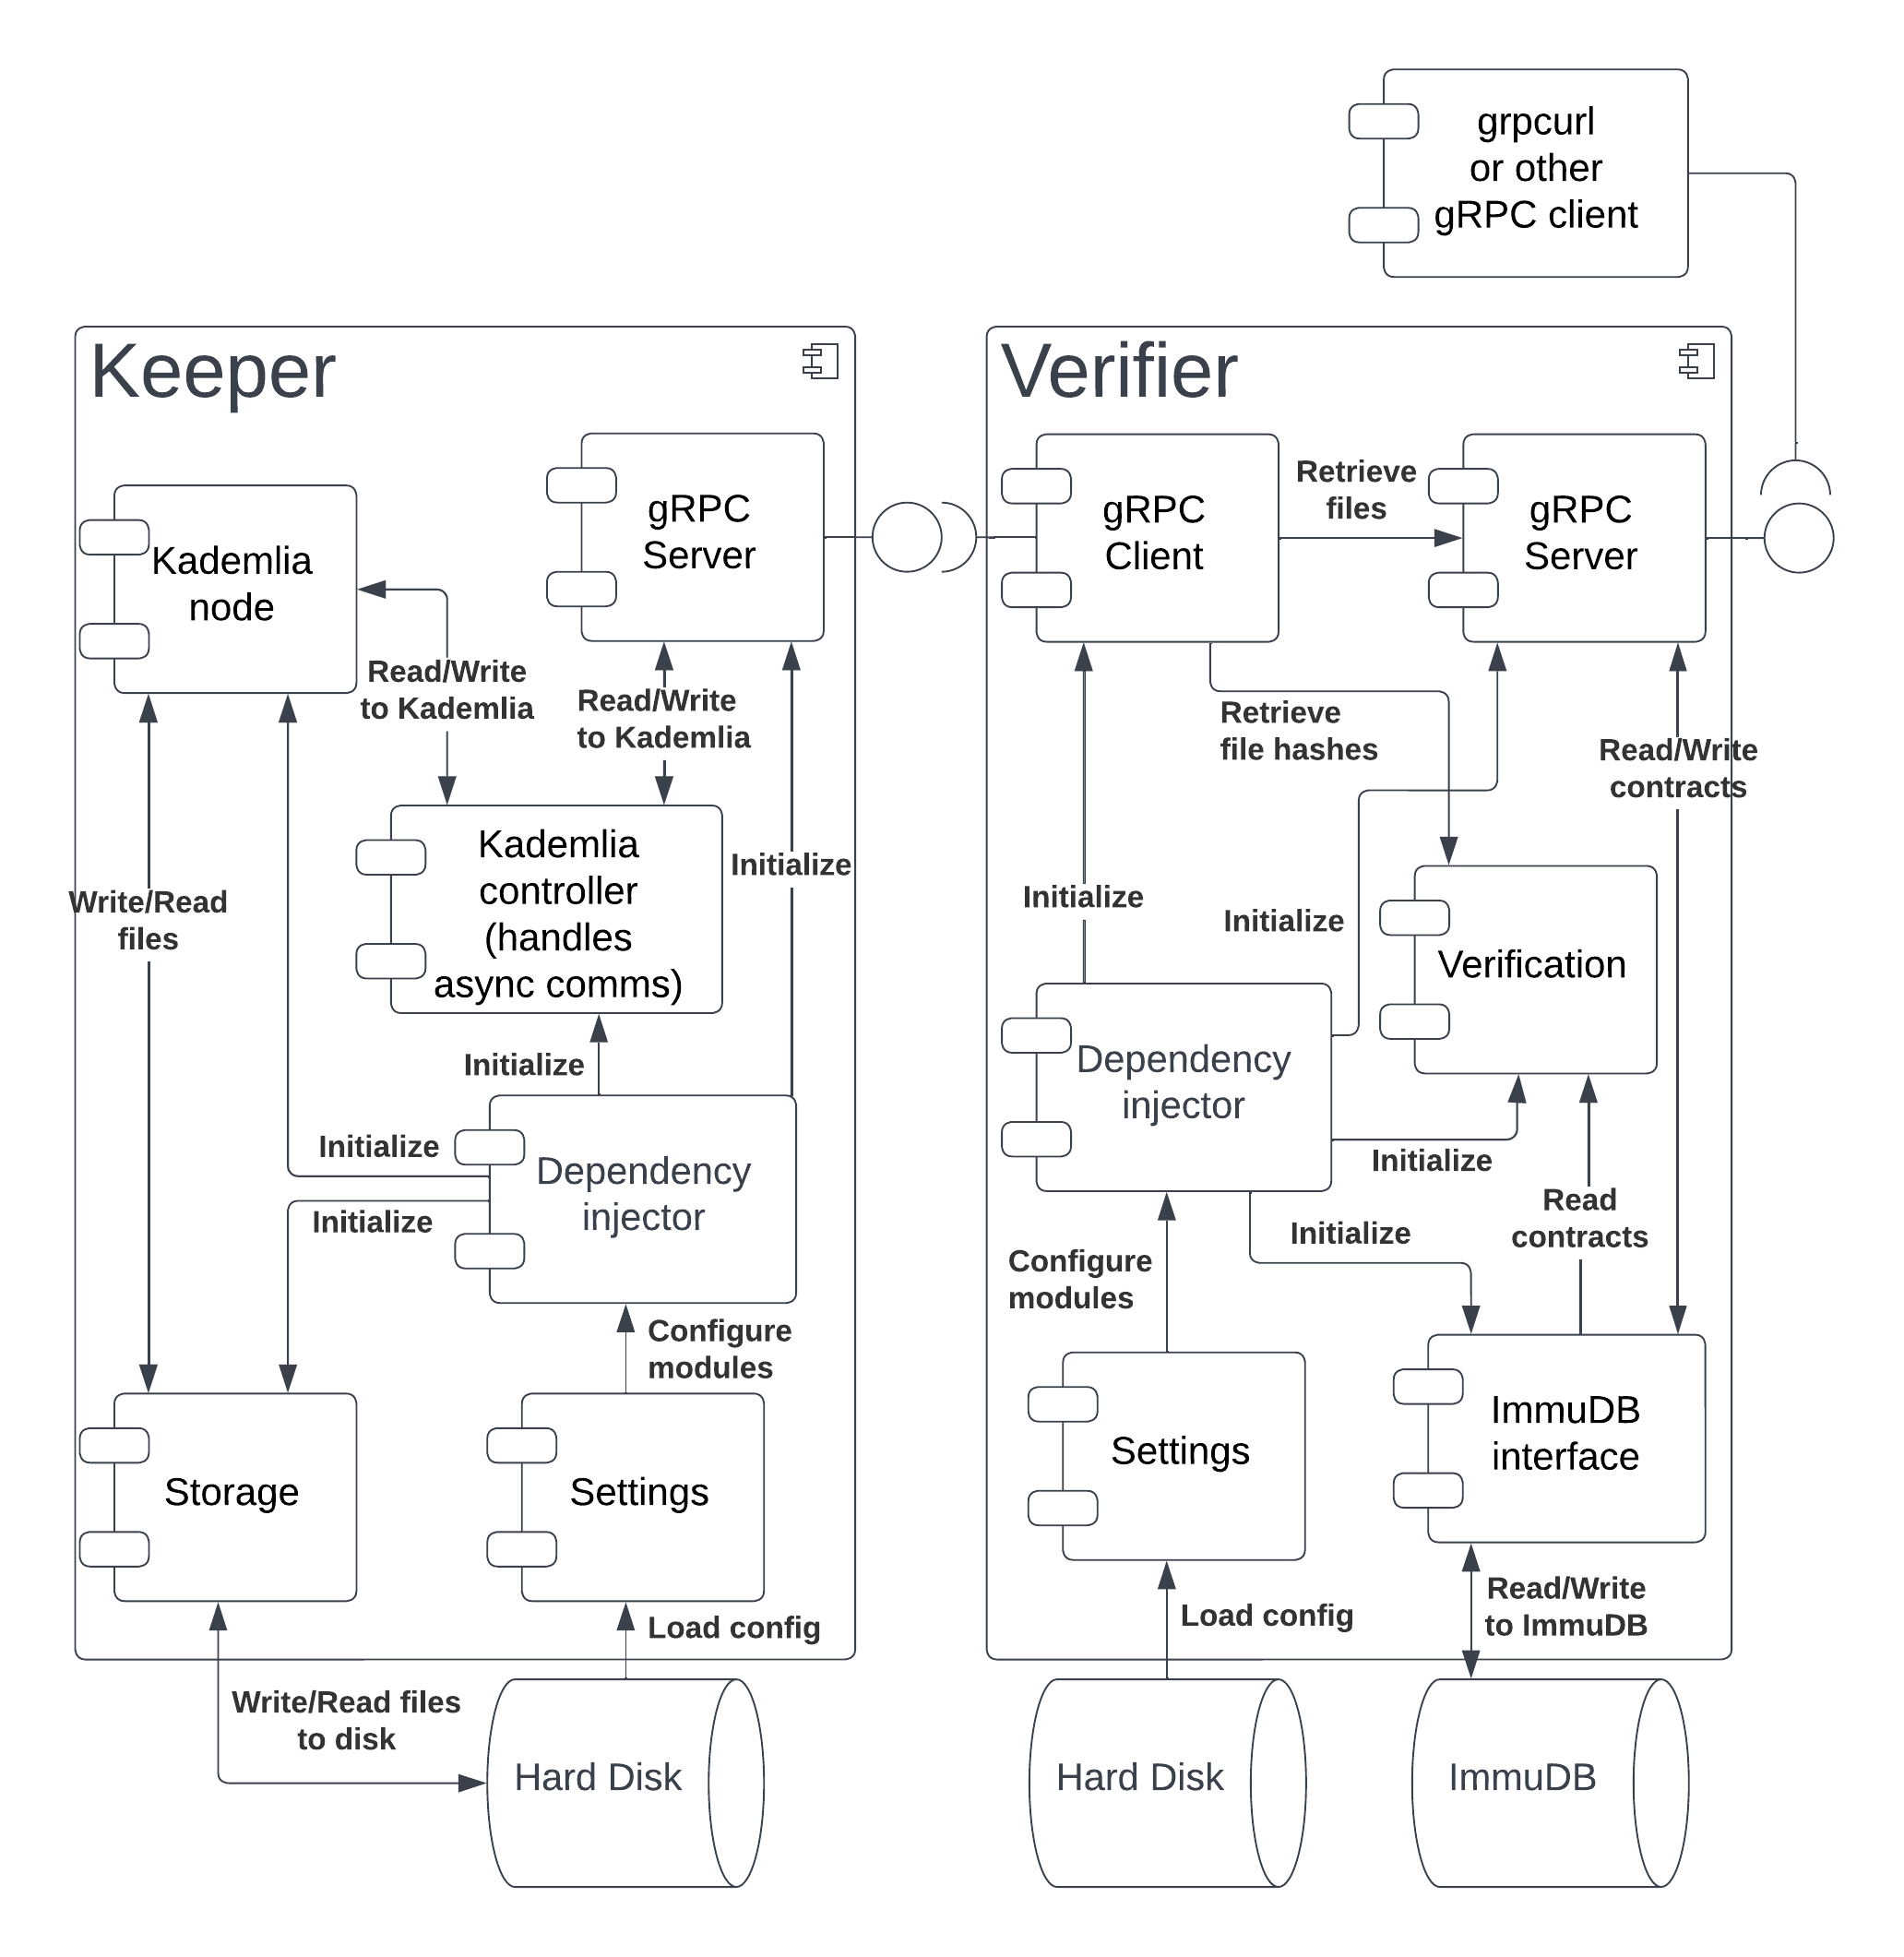
\includegraphics[width=1\textwidth]{gfx/arch-v1.png}
    \caption{Architecture of the system in Version 1}
    \label{fig:architecture-v1}
\end{figure}

\section{Version 2}

Version 2 aimed to work towards decentralizing the verification mechanism.
However, the problem turned out to be more complex than initially anticipated,
which resulted in decentralized verification, but one that is easily attacked.
Luckily during the development of Version 2, we reworked the verification to use a Proof of Retrievability (PoR) scheme,
which allowed us to address the attacks against the decentralized verification mechanism in the future.

In version 2, major flows were addressed.
The storage module was replaced with a custom implementation, which made use of the local disk
using an S3-compatible API.
The Verifier was decentralized, so it was no longer a single point of failure.
The Verifier and Keeper nodes were merged into a single node as two modules,
which would perform both storage and audit operations as seen in \autoref{fig:architecture-v2}.
In doing so, the communication between the Verifier and the Keeper was rewritten to happen over Kademlia.
A new auditing mechanism was introduced, which was based on a Proof of Retrievability (PoR) scheme.
After introducing PoR, we had to rewrite the storage and audit logic to support it
as seen in \autoref{fig:store-procedure-v2} and \autoref{fig:verify-procedure-v2}.
Finally, some attacks were addressed, such as the Sybil attack and the Eclipse attack by introducing
a requirement to solve a cryptographic puzzle upon joining the network.

\begin{figure}
    \centering
    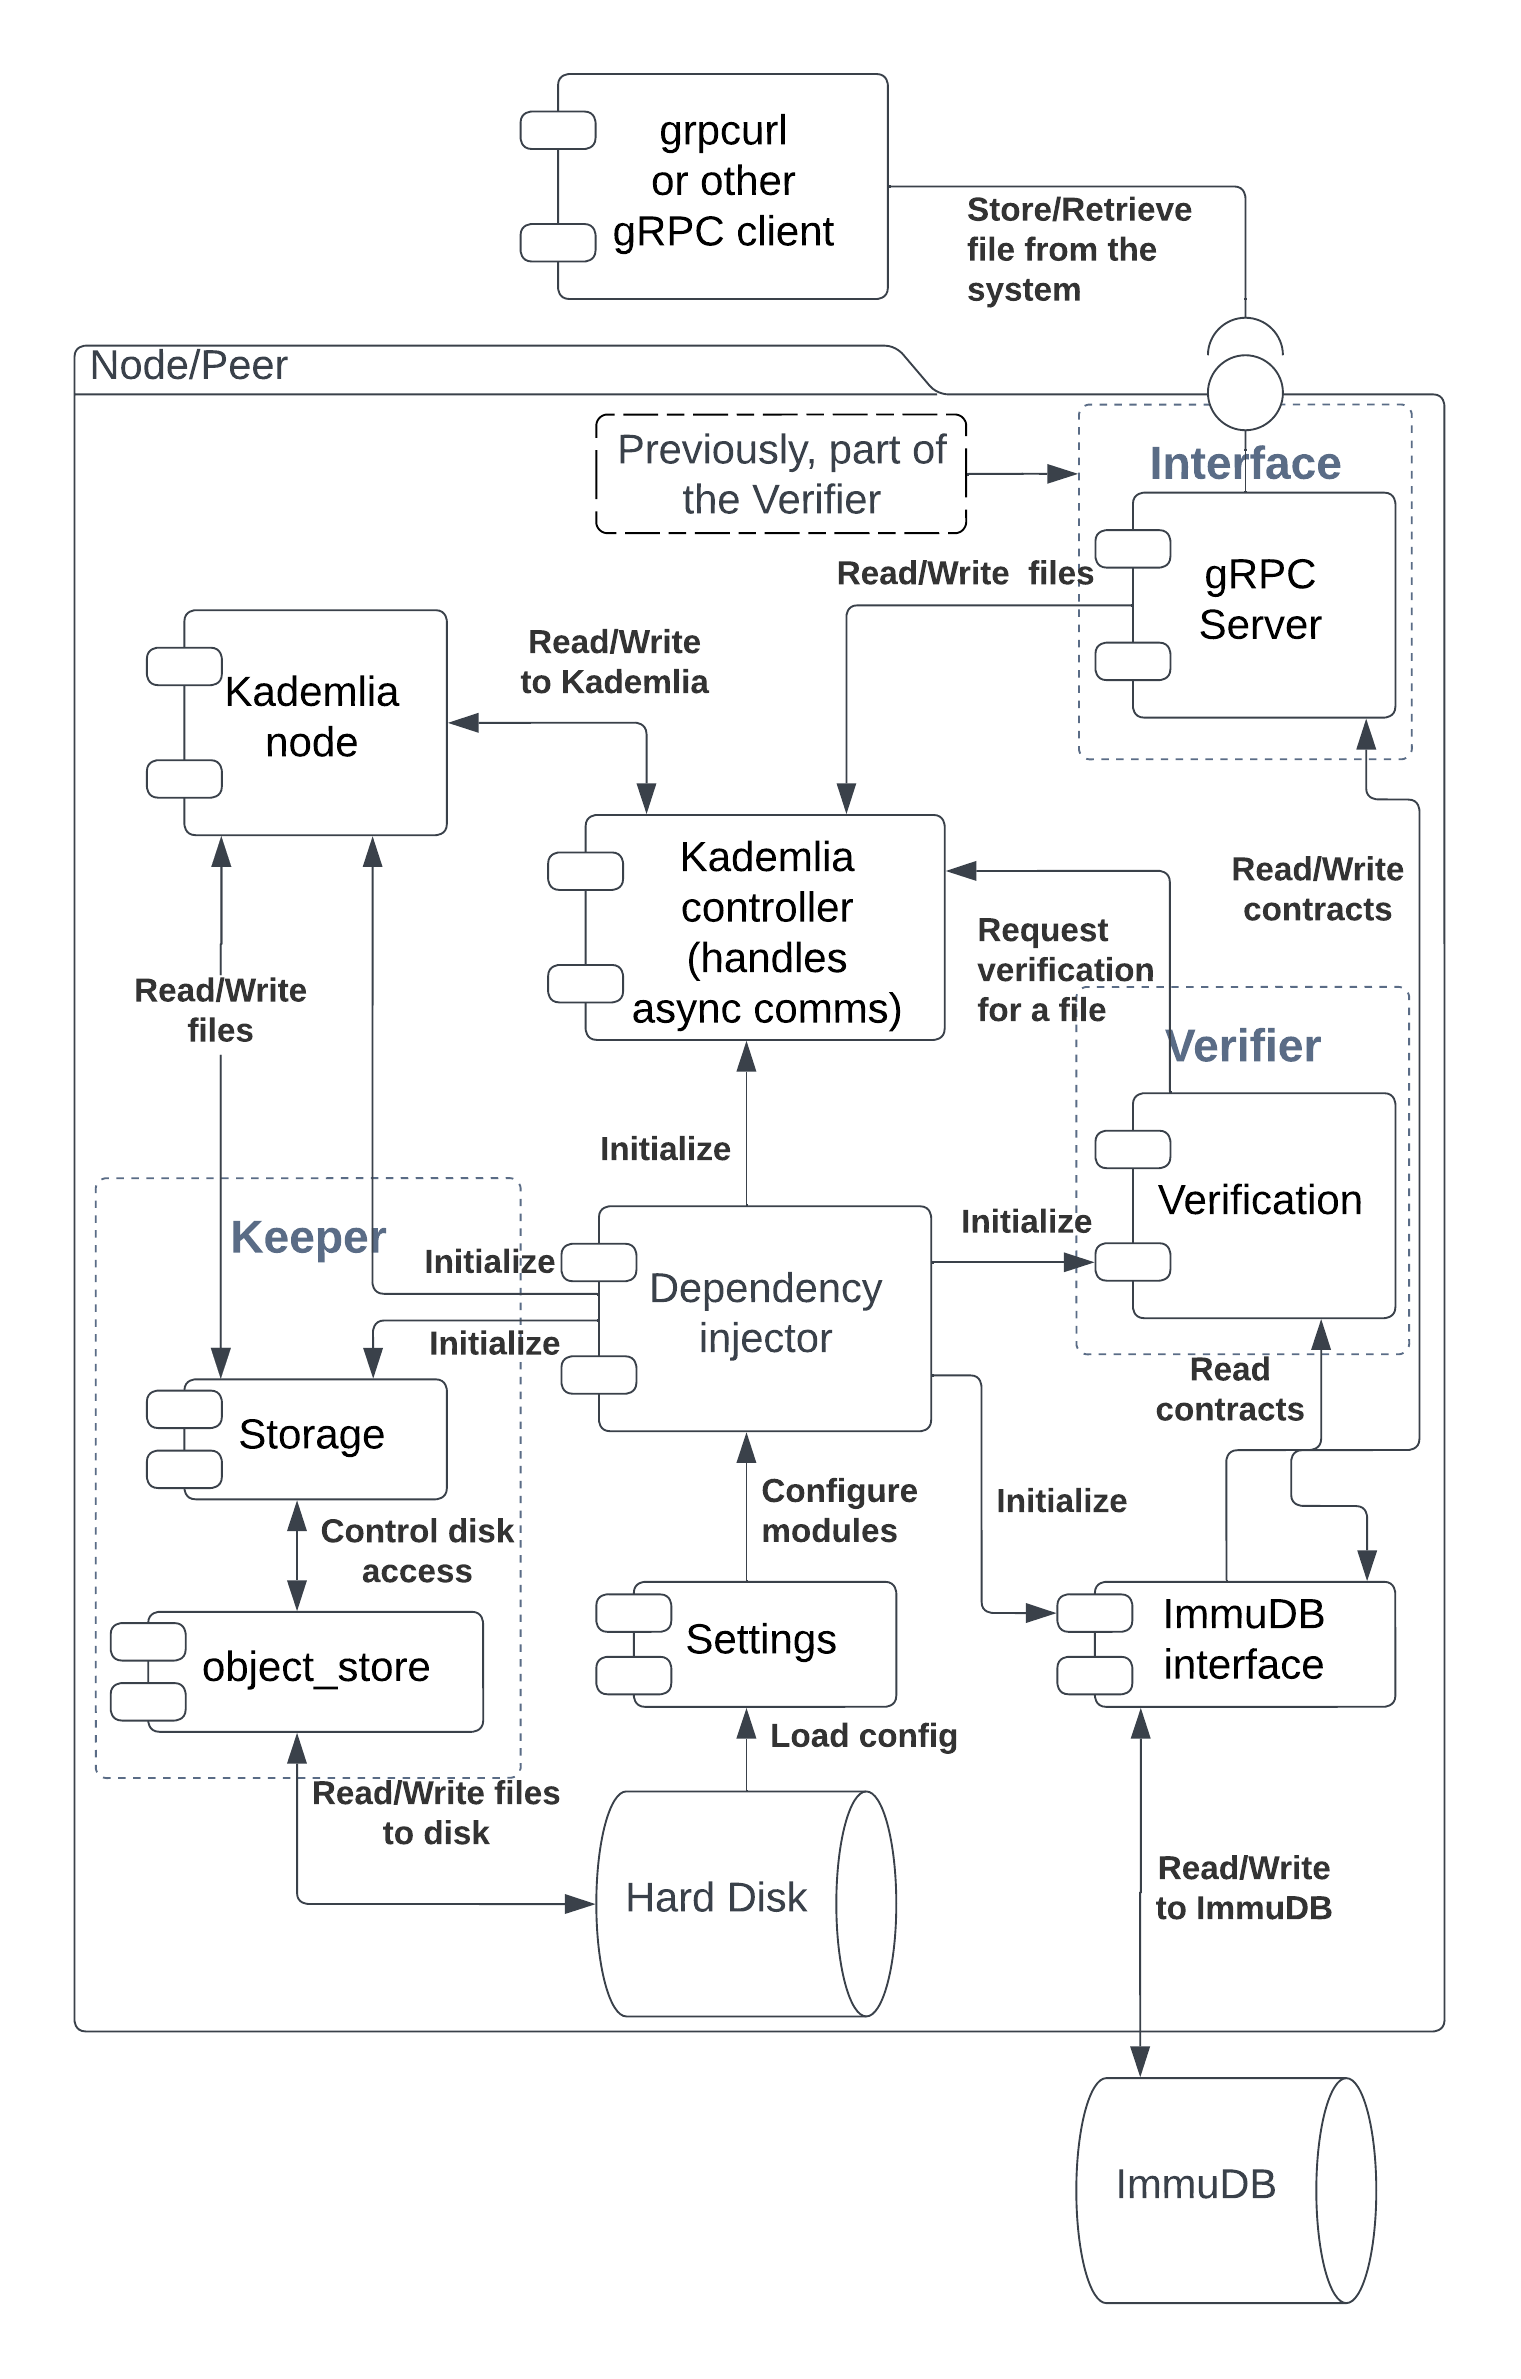
\includegraphics[width=1\textwidth]{gfx/arch-v2.png}
    \caption{Architecture of the system in Version 2}
    \label{fig:architecture-v2}
\end{figure}

\begin{figure}
    \centering
    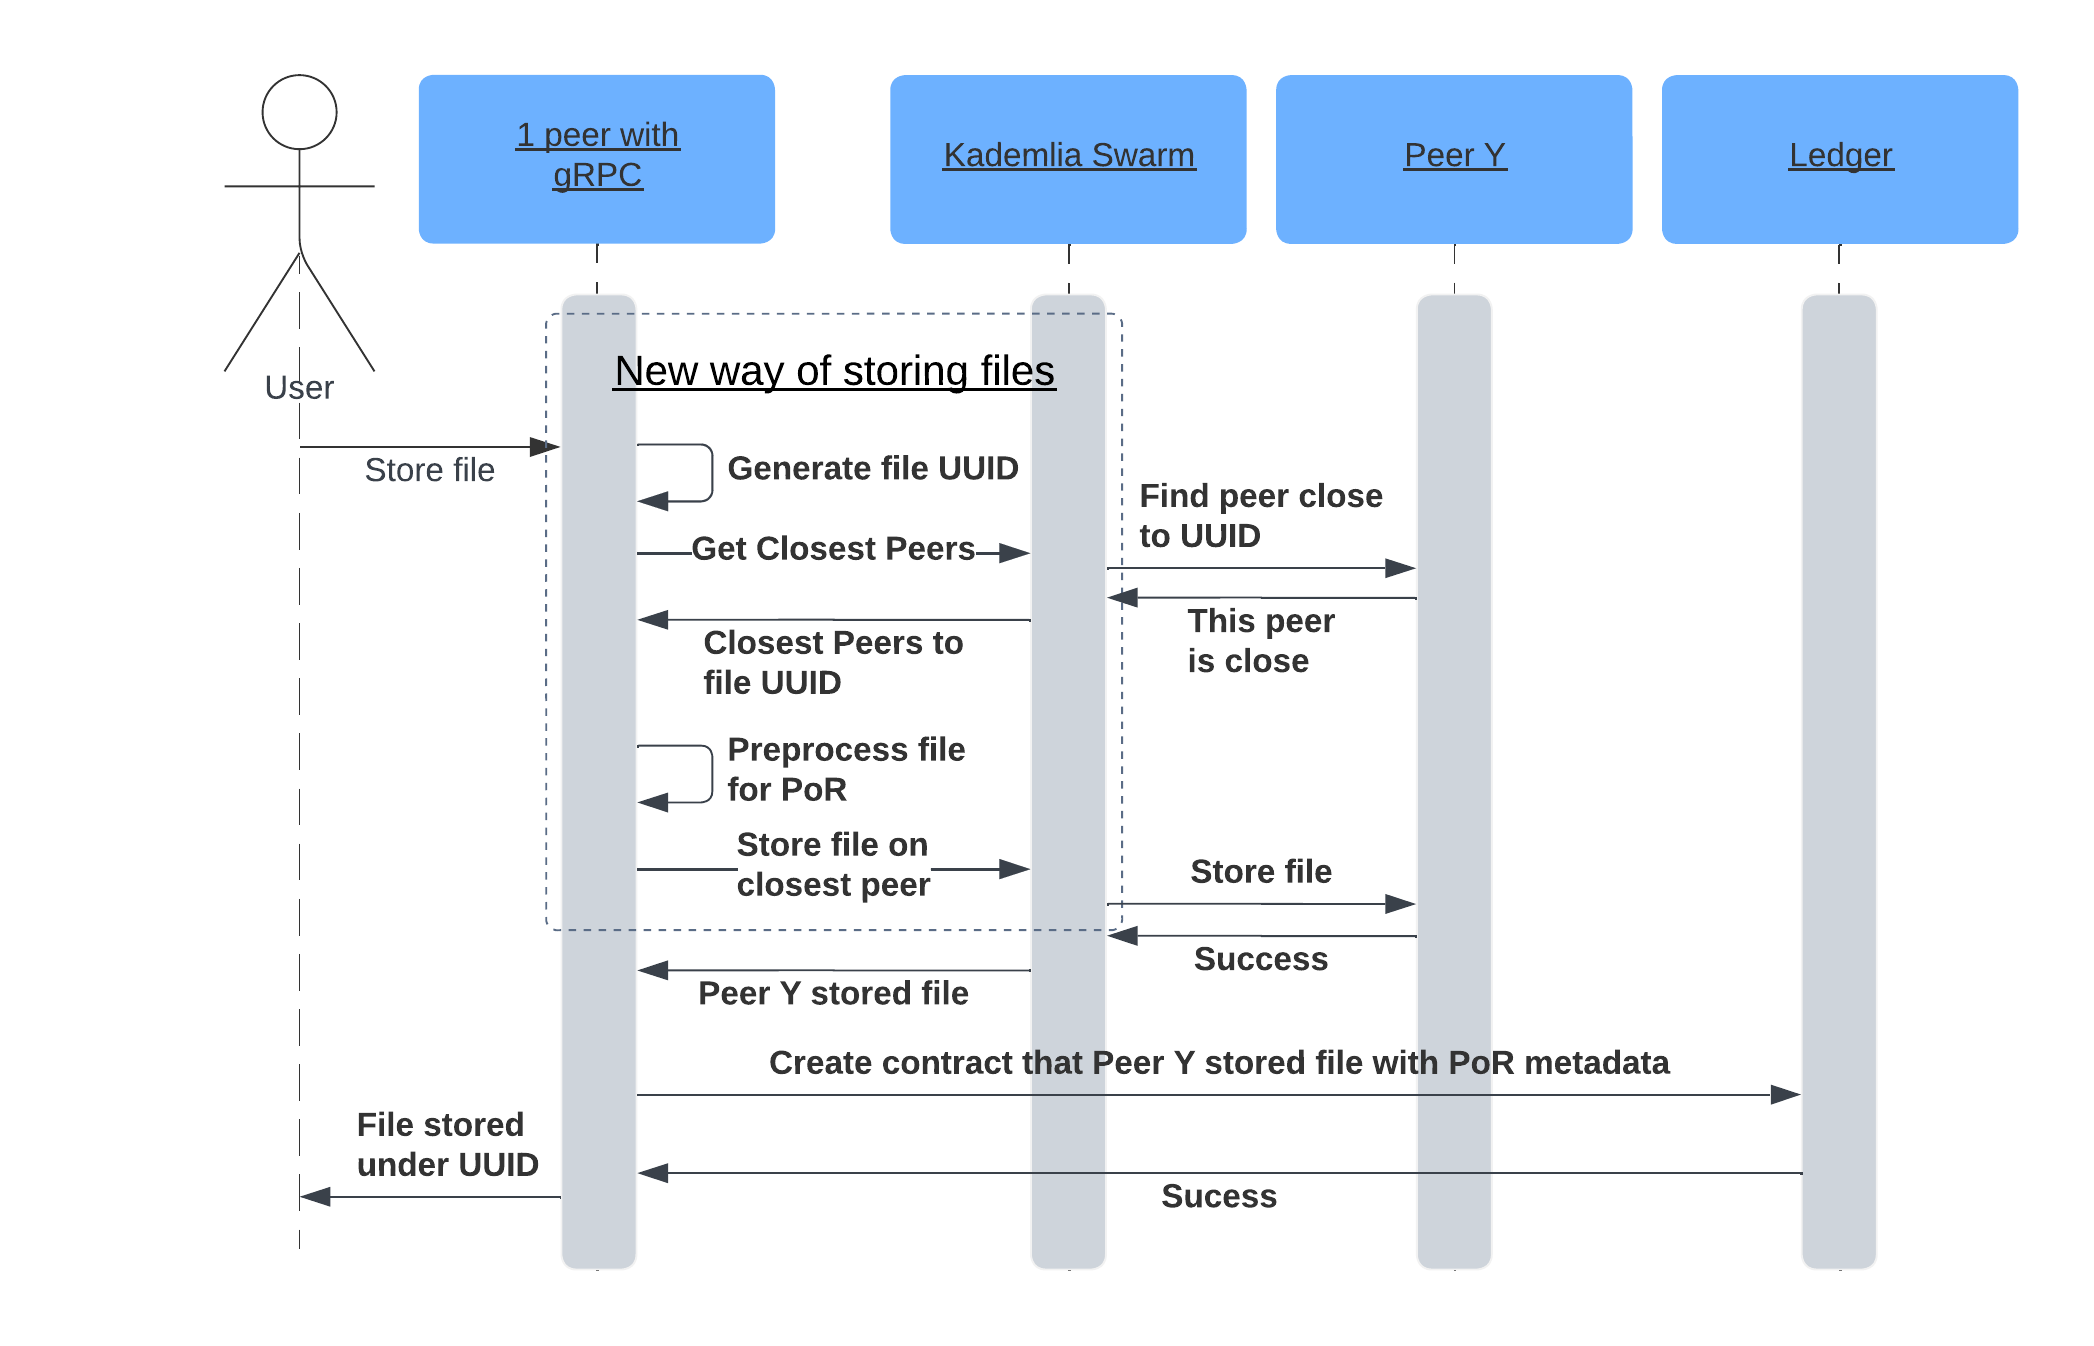
\includegraphics[width=1\textwidth]{gfx/store-procedure-v2.png}
    \caption{Storage flow in Version 2}
    \label{fig:store-procedure-v2}
\end{figure}

\begin{figure}
    \centering
    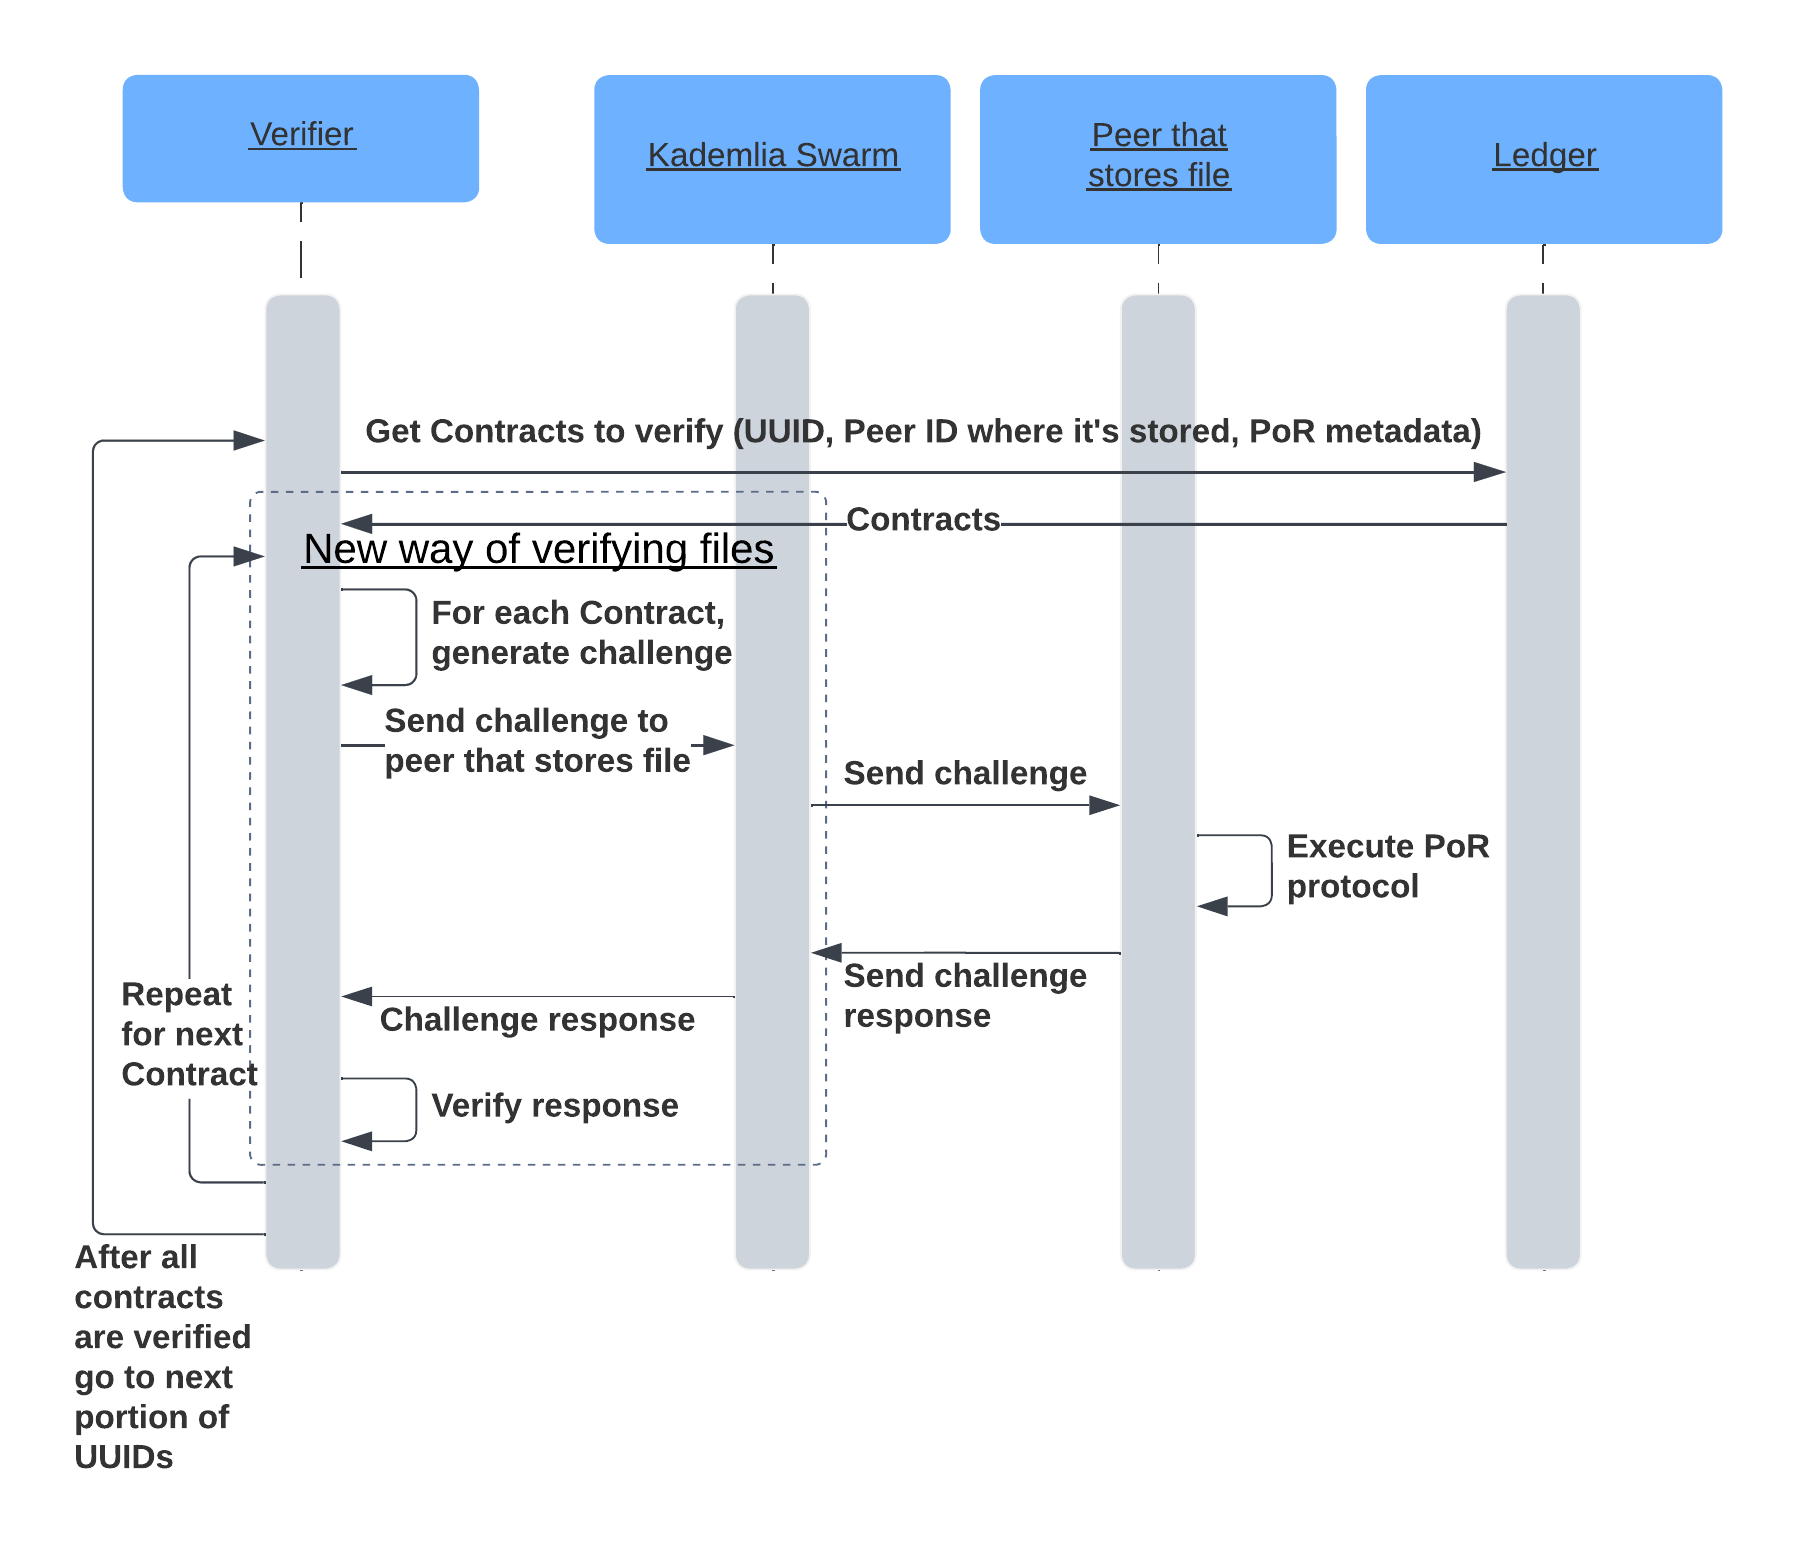
\includegraphics[width=1\textwidth]{gfx/verify-procedure-v2.png}
    \caption{Audit flow in Version 2}
    \label{fig:verify-procedure-v2}
\end{figure}

\section{Summary}

This project started with the aim of creating a fully decentralized storage system with a verification mechanism
to address storage integrity attacks.
In the first iteration we implemented a centralized verifier as a proof of concept,
which we later tried to decentralize only to find the problem to be more complex than initially anticipated.
Decentralizing the verification lead to making the system vulnerable against other kinds of attacks.
However, in the second iteration we improved the verification mechanism by introducing a
Proof of Retrievability (PoR) scheme,
which enabled us to address said attacks in the future.
Our next goal is to implement a defensive mechanism against the attacks we identified in Version 2
by making use of PoR and to evaluate the system's performance and security.
